\documentclass[12pt]{article}
\usepackage{fullpage}
\usepackage{graphicx}
\usepackage[usenames,dvipsnames]{xcolor}
\usepackage{hyperref}
\hypersetup{colorlinks=true,linkcolor=ForestGreen,urlcolor=ForestGreen}
\begin{document}
\begin{center}
  {\Large ECE 651\\ Development Environment Setup}
\end{center}


This tutorial will walk you through setting up your development
environment for ECE 651.  Here are some options and how well they
are supported by the course:

\begin{itemize}
\item Linux: well supported
  \begin{itemize}
  \item Install Virtual Box on your computer and install Linux inside of it.  Note:  if your computer has low resources (e.g. RAM) or is slow, this may be sluggish.
  \item Use an OIT VM (from vcm).  Note that if you want a graphical interface, you will need to use something like VNC. 
  \item Install Linux directly on your computer (possibly dual booting).  Note, we don't walk you through this. 
  \end{itemize}
\item Mac OSX: fairly well supported\footnote{Note: we have not tried this on M1 and do not have an M1 to try it on, but think it should work}.
\item Windows: I believe you can use Linux Subsystem for Windows, but I have never
  used it.  There are Emacs versions for Windows.  There is also
  VSCode for Windows if that is your choice.  You would want to install Java Development Kit (JDK),
  the editor of your choice, and Gradle. 
\end{itemize}

Note that Linux is most directly supported, as I can do a clean
install of a VM, and follow the instructions exactly (with the system
in the same state you will have it if you start from a clean install).
Mac is fairly well supported, as I use a Mac.  However, I cannot start from a clean install
(I am not going to erase my computer), nor are you likely to start from a clean install.  Accordingly,
there might be some differences.   I don't really use Windows, so it is the least supported.  I'll try
to sketch out generally what to do, but you are fairly on your own.

The general overview of what will happen in this walkthrough is:
\begin{enumerate}
\item Install your platform if needed (VirtualBox and/or Linux):
  \begin{itemize}
  \item If you want to install VirtualBox, see Section~\ref{label:VirtualBox}
  \item If you want to use an OIT VM, go to \url{http://vcm.duke.edu/}
    and choose ``Reserve a VM''. Select an Ubutnut 20 image.  Once that is setup, go to
    Section~\ref{setup:git}.
  \item If you want to install go to \url{https://ubuntu.com/tutorials/install-ubuntu-desktop#1-overview}.  Please
    make sure you have a backup of any important data first. Once you have Linux installed, go to
    Section~\ref{setup:git}.
  \end{itemize}
\item Install packages you need: emacs, JDK, gradle, git. Go to Section~\ref{setup:git} directly if you do not need to install a platform.
  \begin{itemize}
  \item You might also want clang/clang-format if you plan to do C (\emph{e.g.}, for 650) in the same environment
  \end{itemize}
\item Setup emacs (install packages, etc) or other edit of your choice.
\item Walk through a small example of how to use Java, gradle, and JUnit.
\end{enumerate}



\section{Installation of VirtualBox}
\label{label:VirtualBox}
VirtualBox is a program that emulates a computer (a virutal machine).  If you
want to go this route, you will basically have a virtual computer running on your computer.
Note that this can be a bit resources intensive, as you need enough memory allocated
to the VM to run its OS and programs.

The first thing you need is
\href{https://www.virtualbox.org/wiki/Downloads}{Virtual Box}, which
will run a virtual machine on your computer (effectively, it will
pretend to be a computer).  On the page linked above, you should see a
section near the top called ``VirtualBox 6.1.30 platform packages''
with a list of operating systems under it.  Choose your OS to download
the appropriate Virtual Box installer.  Once you have downloaded the
Virtual Box installer, install it just like you would any other
program on your computer.

Next, you need to go to  \href{https://ubuntu.com/download/desktop}
and download Ubuntu 20.04.3 LTS (should be at the top of the page).  This download may take a long time,
as it is a 2.9 GB.  

Now, you are ready to start Virtual Box, and set up a VM.  Open the
Virtual Box program you just installed, and you should see a screen
like this (though it may look slightly different as Virtual Box has a new version since we
originally wrote this):

\begin{center}
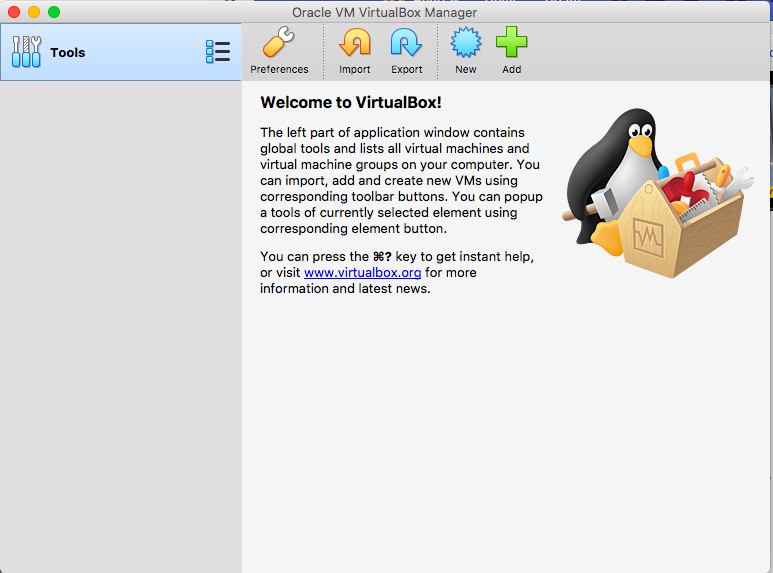
\includegraphics[width=5.0in]{vbox1.png}
\end{center}

In the upper bar, towards the right is a ``New'' button (with a blue
spiked circle icon).  Click on that button and you will get a dialog
to fill in some basic info.  Fill it in as follows:
\begin{itemize}
\item Name: ECE 651
\item Machine Folder: (whatever it gave you by default)
\item Type: Linux
\item Version: Ubuntu (64-bit)
\end{itemize}

The next screen will prompt you for memory size.
What you put here  depends on how much RAM your computer has.
People have had problems installing with less than 2GB.  3GB
is not too bad.  If your computer has 8 or more GB of RAM,
we recommend giving your VM at least 4GB.
If you have a lot of RAM, giving even more can be great.
The coloration under the slider indicates how much of a problem
it will be for your computer to use that much of its RAM for the VM.
If you pick things in the orange or red ranges, you may have trouble
with anything outside the VM.


The next screen will  ask about making a virtual hard disk.  You want to choose
``Create Virtual Hard Disk Now'' (this should be checked by default).

Once you click ``Next'' you will be prompted for the Hard disk file type,
the default (``VDI VirtualBox Disk Image) is fine, so just click ``Next''.

The next screen will ask you how to stor it, again the default
(``Dynamically allocated'') is fine, so just click ``Next''.

On the next screen, you will be asked for where to store the disk file
(the default is fine), and how much space to put in the disk.  The
default is 10GB, which is probably too small.  You may be able to get
by with it if you need to, but might run out of space later in the
semester (you can resize the disk with a tool if you need).  If you
have plenty of free disk space on your computer, I would recommend
going up to 15GB or even 20GB just to be safe.

After you finish creation, you should be back ot the main Virtual Box
screen with the information for your newly created VM displayed:

\begin{center}
  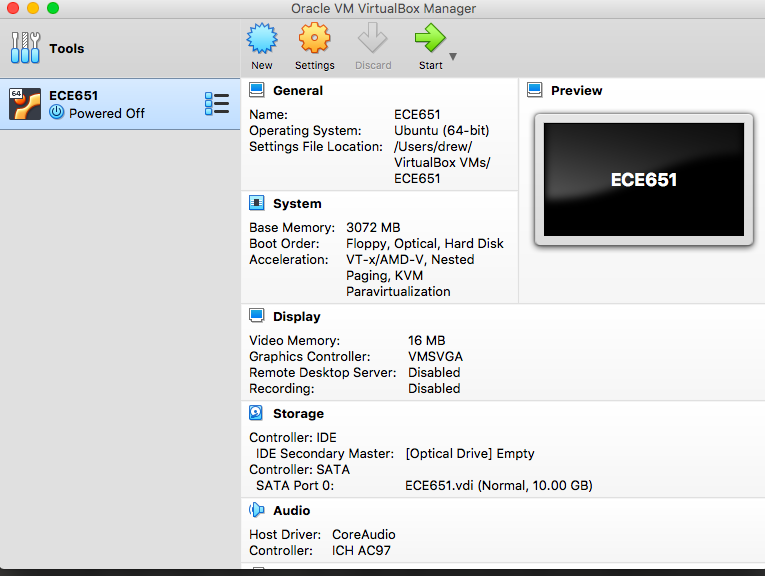
\includegraphics[width=5.0in]{vbox3.png}
\end{center}

Before you power on the VM, you need to tell it to use the Ubuntu ISO
as its CD drive.  Go to ``Settings'' at the top, and then ``Storage''.
On the left, under ``Controller IDE'' select the CD drive which is
labeled ``Empty''.  On the right is a small icon of a CD drive (near
where the tool tip is displayed in the screen shot below).  If you
click on this icon, you should be able to ``Choose/Create Virtual Optical
Disk File'' and then select the Ubuntu ISO you downloaded previously.

\begin{center}
  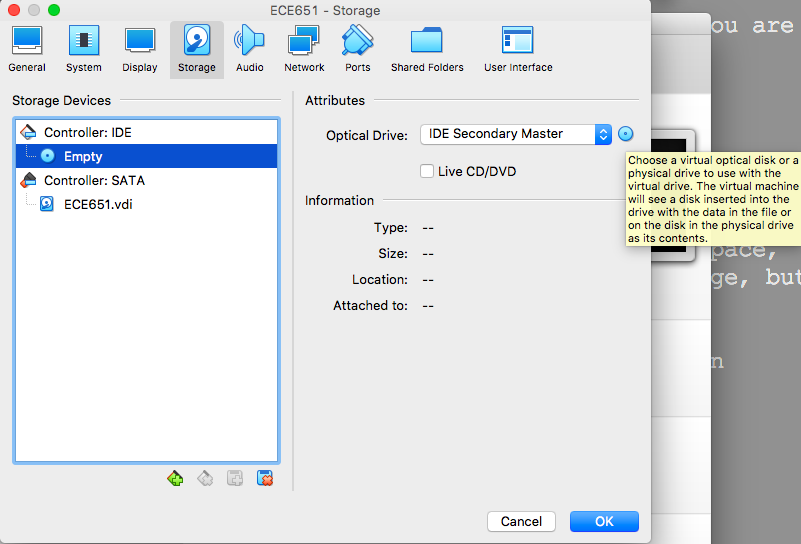
\includegraphics[width=5.0in]{vbox4.png}
\end{center}


Note that if you use a resolution larger than 1920x1600 you will probably
need to adjust the video memory upwards too if you want to use your VM
full screen.  I use an 40 inch monitor at a 3840x1600 resolution, so I change
my video memory to 64MB.  It turns out my Mac has a 5120x2880 resolution, so
needs 128MB of video memory to go full screen.  That computer is also 7 years old,
so VirtualBox is really sluggish in full screen. If you don't use a very large resolution, you
can skip this.  If you don't have your video memory high enough for a resolution
you try to use, you'll end up with the screen being black until you shrink it back down.

You can also (but do not have to) give VirtualBox more than one CPU
under System $\rightarrow$ Processor. 

After you accept your changes, you should be back at the main screen.
Click ``Start'' (with the green arrow in the upper right corner) to
boot the VM.  You should see it boot up, and then give an Ubuntu
loading screen.  Followed by an install menu with ``Try Ubuntu'' or
``Install Ubuntu'' buttons.  Choose ``Install Ubuntu'' (don't worry,
it will only install in the VM, everything on your regular computer
will be left alone, as long as you are doing this in Virtual Box).

On the next screen, choose your keyboard layout.  The screen after
that asks you if you want a normal installation of a minimal
installation.  You can choose either, but the normal will take longer
and give you a lot of things you don't need for this class (like a
music player, a word processor, etc).  Do check the box for third
party drivers at the bottom though.

The default option on the next (Erase disk and install Ubuntu) is fine
(again, this just erases the virtual disk, not your real disk).  Hit
``Install Now'', and then ``Continue''.  Next you will pick your
timezone, and then a user name and password.  Hit ``Continue'' then
you will wait a while as it installs everything.

Unless there are any problems, you should wait a while (or
maybe get up, get a snack, go for a walk,... it will take a while) as Ubuntu
copies and installs its files, then get a box asking you to restart
now.  After you click that box, Ubuntu will take a moment to shut
down, and then prompt you with a screen to ``Please remove your
installation medium, then press ENTER''.  You should be able to just
press ``Enter'' as the installer should have automatically ``ejected''
the virtual disk.

The VM should reboot and after a brief bit of loading, display a
screen for you to select which user you want to login as (there should
be one choice, which is whatever user name you selected during setup).
After you login, you will need to click through a few more setup
screens.  There is a ``Skip'' button in the upper right to go past
connecting other accounts.  You can also just hit ``Next'' (same place)
to skip setting up LivePatch and the other few screens.  Once you get to the last
screen, hit ``Done''.

You probably have a ``Software updater'' pop-up waiting for you. If so, go ahead
and hit ``Install Now'' to update the software, and type your password. Wait for
it to finish before you proceed.  This update probably takes several minutes,
as it is going to do any updates to any packages that have had changes since
this version of Ubuntu was released.  

Now click the 9 dots in the lower left corner (which says ``Show
Applications'' when you mouse over).  You should have several rows
of icons, once of which (in the bottom right) should say ``Ter..'' and
have a black square with a white \verb+>_+ in the top left as its icon.
Clicking on that should bring up a terminal.    In that terminal, do

\begin{verbatim}
sudo apt install gcc make perl xterm
\end{verbatim}
You should be prompted for your password (type it) and then asked if you want
to proceed.  Hit ``y'' and wait while these packages install.  

I prefer xterm to the default Ubunut terminal.  If you type
\begin{verbatim}
xterm &
\end{verbatim}
in your current terminal, a new terminal will pop up that is an xterm.
We'll adjust its configuration later (once you have git installed, and
we can get a file from git).  For now, you may wish to right clikc the
XTerm icon on the left bar and choose ``Add to Favorites''.

Now, you will want to take a second to install the ``Virtual Box Guest
Additions'' (which is software to add features specific to running
inside Virtual Box.  Go to the ``Devices'' menu, then ``Insert Guest
Additions CD Image''.  When you do this, you should get a message box
asking if you want to run what is on the CD.  Accept this, and wait a
minute while it installs.  Then it will tell you to press Enter when
you are done.  Once this is installed, you will want to restart the VM
for the updates to take effect. To do so, go to the menu in the upper
right (that looks like a power button) and choose Power Off/Logut,
then Power Off, then Restart. After restart, you will be able to (among
other things) resize or full screen the VM window, and have it use the
entire new window size.  You might wish to full screen the VM (Host+F.
On Mac, Host defaults to left command.  On Windows, right control).


We will briefly note that if you are away from using the VM for a
while, the screen in it will lock.  If you click in it, it won't show
a password box---just start typing your password and the box will
appear.  You might want to go to the ``Devices'' and choose ``Shared
Clipboard'' and then select ``Bidirectional'' if you want to be able
to copy/paste between the VM and the host.

Note that in Linux, copy is ``highlight'' and paste is ``middle click.''
If you have a 3 button mouse, this should not be a problem.  If you have
a track pad, you may wish to bind a key on your keyboard (that you do not
use often) to emulate middle click.  If your host is a Mac,
you can run the  \verb+mac-paste.sh+ script that we have included
in the git repository you will clone shortly.  This script will rebind right option
to be middle click inside the VM.  If you are using Windows (or want
a different key on Mac), you can adjust the script to whatever key code you want
and then run it.

One quick note about the virtual machine: this software is emulating
an entire computer.   If you just close the VM, it is like ripping the power
cord out of the wall on a physical computer---the OS has no time
to flush its disk caches.  Doing so can lead to corruption of files.
To shut your VM down, you should go to the drop down in the upper right corner
of the guest OS (Linux inside the VM) and Power Off/Logout, and select
Power Off then shut down.

At this point, you should have a bare, but functional Linux environment.
Next we will want to install git, so we can clone the git repo for this
tutorial, which has several useful files.

\section{Install Git + Clone Repo}
%\label{package:linux}
\label{setup:git}
Next we need to install a bunch of packages.  On Linux, this can be done with
the \verb+apt+ package manager.  On Mac, this can be done with Homebrew.
On Windows, you are going to need to download and install a bunch of things yourself.
For Mac and Linux, we have written some scripts that will install the appropriate
packages for you.  They are in a git repository, so the first thing you should
do is install git.

\textbf{For Linux:}
\begin{verbatim}
sudo apt install git
\end{verbatim}
\textbf{For Mac:}
If you try to run git and it is not installed, you should be prompted to install it.
\textbf{For Windows:}
Go to \url{https://git-scm.com/book/en/v2/Getting-Started-Installing-Git} and look for ``Installing for Windows''.


Now is a good time to setup some important git info too.  You will
need to run these two commands (put in your own name and email, as you
want them to appear in commit messages):

\begin{verbatim}
git config --global user.name "Your Name Here" 
git config --global user.email "Your Email Here"
\end{verbatim}

You may also want to do

\begin{verbatim}
git config --global credential.helper store
\end{verbatim}

This will make git remember your gitlab password.  Note that it
unfortunately stores it in plain-text, so you should only do this if
the computer you are working from is completely secure.

Next, you can either just clone our repository, or you can make a fork
of it.  If you fork it, you will have your own version of it, and can
push changes to it.  Why would you want to do that?  We are going to
have a brief section on ``upping your Emacs/git game'' and you may
wish to play around with it.  If you want to fork, go to
\url{https://gitlab.oit.duke.edu/adh39/ece651-dev-setup} in your web
browser.  Choose the \textbf{fork} button in the upper right, and
follow the instructions.  If you do this, get the ``clone'' URL from
your own project and use it in the next step instead of ours.


Now do:
\begin{verbatim}
git clone https://gitlab.oit.duke.edu/adh39/ece651-dev-setup.git
\end{verbatim}

If you cd into ece651-dev-setup, you will find a some shell
scripts, and a doc directory with a copy of this pdf (and its \LaTeX source).


If you are on Linux, run \verb+packages-linux.sh+ script.  Note that this script
will ask if you want to update your DNS settings. VirtualBox has some weird default
DNS setting that make name resolution slow.  If you choose yes, you will get your DNS
changed to use Google's DNS servers.

If you are on Mac, run the \verb+packages-mac.sh+ script.
If you are on Windows, you will need to install the following:
\begin{description}
\item[Gradle] Go to \url{https://gradle.org/releases/}. Choose version 7.3.3.  It is \emph{not}
  the latest, but more recent versions changed the layout of projects in ways that many tools
  do not yet support.
\item[Emacs] Go to \url{https://www.gnu.org/software/emacs/download.html}
\item[Java Development Kit (JDK)] Download and install \url{https://download.java.net/openjdk/jdk16/ri/openjdk-16+36_windows-x64_bin.zip}
\item[Clang format] If you want this to support C auto formatting (as
  in 551), you are on your own here, but
  \url{https://llvm.org/builds/} might be a starting point.
\end{description}

Before you proceed, \textbf{close and reopen} your terminal. The install scripts added
things (like Gradle) to your PATH in your login files.  These will take effect when
you reopen your terminal.

\section{Emacs Setup}
Now, we need to do some Emacs setup.  Emacs has its own package management
and configuration.  We need to install some Emacs packages and configure them
to have the nice set of features you are used to.  For Linux and Mac this is
done for you if you just run the \verb+emacs-config.sh+ script we have provided.

If you are on Windows, you might look into how to run a bash script.  If not,
this works through a four step setup: (1) a minimal config file that sets
up package management (2) installation of packages (3) installation of a custom
package (4) setup of the main configuration file.  You could probably work through
them one by one by hand. 


Please note that this configuration script assumes you are running in a new
setup, and will \textbf{completely overwrite} your emacs configuration.  If you have
things there that you want to keep, please back them up first.  You
will need to integrate them manually into configuration file
afterwards.

Now run the setup script:
\begin{verbatim}
./emacs-config.sh
\end{verbatim}

At this point, you should have Emacs all setup and ready to try out.


\section{Getting Started With Gradle}

Next, let us take a moment to get acquainted with our Emacs setup for
Java, and Gradle (which one of the two most commonly used build system
for Java).  Let us make a directory for ``try-emacs'', and initialize
a gradle project in it.  \textbf{Note:} many of the tools that we use will consider ``top of the
git repository'' as the top-level of the project.  Accordingly,
we'll make this a git repository even if you don't need to commit
it to git.  If you don't, then you will end up having to specify
the project directory manually, or get some weird behavior.


\begin{verbatim}
cd ~
mkdir try-emacs
cd try-emacs
git init
gradle init
\end{verbatim}


Gradle will ask you some questions, you want to answer them
as follows (you don't need to type what is in parenthesis, those are
just there to make sure the number matches what you see)
\begin{description}
\item [type of project] 2 (application)
\item [implementation language] 3 (Java)
\item [Split Functionality across multiple subprojects] 1 (No)
\item [build script DSL] 1 (Groovy)
\item [Generate build using new APIs and behavior] no
\item [test framework] 4  (JUnit Jupiter) 
\item [project name] enter (default is fine)
\item [source package] edu.duke.ece651.example
\end{description}


If you do ``ls'' you will see some gradle configuration files,
and an ``app'' directory.  There is not a top-level build.gradle file
here, but we will need one to work with our test coverage tool.
In the ece651-dev-setup git repository there is a file that will work, so
\begin{verbatim}
cp ~/ece651-dev-setup/top-level-build.gradle build.gradle
\end{verbatim}

The build.gradle file is analagous to (though very different from) a Makefile.
Newer gradle versions require that the project be setup with subdirectories
for each subproject (even if the project doesnt have subprojects, and is just
one big project).   Our ``app'' directory is the subproject, which is where most
stuff happens. Next, cd into it

\begin{verbatim}
cd app
\end{verbatim}

We will make a few small changes to the build.gradle here as well.
Open that file in emacs (or your other editor of choice), e.g.

\begin{verbatim}
emacs build.gradle &
\end{verbatim}
Note that the above will run emacs in the background.  If you are in VirtualBox, you
will get graphical-mode Emacs by default, so this will cause your terminal to give you a prompt
and let you keep using it.  If you want terminal-mode emacs, do \verb+emacs -nw build.gradle+.

In the \verb+dependencies+ section, add
\begin{verbatim}
   testImplementation 'org.junit.platform:junit-platform-launcher:1.6.2'
\end{verbatim} 
And then at the end of the file, add this:
\begin{verbatim}
test {
    testLogging {
        showStandardStreams = true
        exceptionFormat = 'full'
    }
}
\end{verbatim}
The first of these is needed to make clover (the code coverage tool)
work properly with JUnit.  The second will make it so that  during testing,
you will see any output you create on stdout and/or stderr, and
fully detailed exception traces.

Before going any further, run
\begin{verbatim}
gradle build
\end{verbatim}

to make sure that everything is OK with your gradle file.  This will
take a while the first time, as gradle will download various
things your project depends on (clover, junit, etc). It will go
much faster the next time.



 If you look in the \verb+src+ directory, you
will see that it is organized like this
\begin{verbatim}
 - src 
   | 
   +--main 
   |  | 
   |  +-java 
   |    |  
   |    +-edu
   |      |
   |      +-duke
   |        |
   |        +-ece651
   |          |
   |          +-example
   |            |
   |            +-App.java
   +--test 
      |
      +-java 
        |  
        +-edu
          |
          +-duke
            |
            +-ece651
              |
              +-example
                |
                +-AppTest.java
\end{verbatim}

The \verb+main+/\verb+test+ division separates the main code (the
stuff you actually want to run and deploy) from the testing code.
Inside each of those is a \verb+java+ directory since our code is in
Java.  If we had other languages, we could put other directories
alongside those for the other languages.  Each of those directories
then has a path corresponding to the package name.  

In Java, classes are organized into packages.  You will quickly become
familiar with many standard packages, such as \verb+java.util+ and
\verb+java.lang+.  However, the code you write also should be in
packages.    Proper naming of a Java
package, starts with the internet name of the organization
that created it, written in reverse.  In particular, this means that
any package you write for this class should start with
\verb+edu.duke.ece651+, for example.  The directory structure
mirrors the package name, with each component (as separate
by a dot) being a directory.  So the code for the package
\verb+edu.duke.ece651.example+ will be in the directory
\verb+edu/duke/ece651/example+.

\section{Emacs for Java}
Most of your favorite editing commands from 551 will work just as you expect,
including auto-complete from company (complete-anything)!
However, we've set you up with some Java-specific features (mostly from
the lsp-java and dap-java packages). We are going to go give you an introduction
to those here.

Note that we give you a quick reference in Section~\ref{Sec:QuickRef}.  This
quick reference covers all the commands we discuss in this walk-through,
as well as a few others that are useful, but we don't think require
much explanation (\emph{e.g.}, ``format buffer'').


Let us create a file called \verb+Thing.java+ inside our package.  If you don't
already have emacs open, 
\begin{verbatim}
emacs src/main/java/edu/duke/ece651/example/Thing.java 
\end{verbatim}
If you do, then you can hit C-x C-f and type the filename in the minibuffer to open it.

Hopefully from 551, you remember that you should use TAB completion
extensively in the shell, or in Emacs i.e., you should have typed the command as:
\begin{verbatim}
emacs sr(TAB)m(TAB)j(TAB)(TAB)(TAB)(TAB)(TAB)Thing.java
\end{verbatim}
or similarly tab completed the name of what to open if you were using C-x C-f.


Note that if you add an \verb+&+ to the end of the command,
bash will run emacs in the background and give you the prompt back.
This works fine with graphical emacs, and leaves the shell available
in another window in case you need it.  If you are running on an OIT VM,
you probably want to give \verb+-nw+ to emacs to ensure it does not try to run
across an exported graphical connection.

At this point, you should be looking at an Emacs window with a dark
background\footnote{We set you up with the Dracula theme by default.
  If you want to change the theme, please see the instructions at the end
of this document}, and nothing in it.

For the very first Java file that you open, the LSP-java package
should need to download a bunch of stuff.  This should only happen one
time, but takes a while.  It is going to ask you what server you need
to install (you might have some other message, but clicking into the
window or doing anything should prompt you), and you should type
\begin{verbatim}
jdtls
\end{verbatim}

This should pop up a buffer \verb+*lsp-install.sh*+ which will show
you the install progress (M \verb+>+ if you need to get to the end of the buffer
to follow what it is doing).  Note that it will take a few minutes.


When this finishes successfully, it will prompt you with
\begin{verbatim}
Things.java is not part of any project. Selection action:
i ==> Import project root ~/try-emacs/.
I ==> Import project root by selected root directory interactively.
(some other options).
\end{verbatim}
When you open a file from a new project (meaning anything that
LSP-java does not know about the project setup yet), you will get
prompted for how LSP-java should identify the project.  You will
typically want either 'i' (if the listed directory is correct) or 'I'
if it is not.  Here ``correct'' means the directory which has
everything for this project and nothing from any other project
(typically where your build.gradle is).  This project setup selection
will put everything under the directory into this project.  A few
important things can go wrong here:
\begin{itemize}
\item If the directory listed for 'i' (or that you pick with 'I') is
  too high up (e.g., your entire home directory) then code you write
  for other projects will be treated as part of this project.
\item If the directory listed for 'i' is too deep (\emph{e.g.}, is inside
  the src directory) then various tools will not be able to find all the
  parts of the project.
\end{itemize}
If this the information under the ``i'' option is \verb+~/try-emacs+ then
you should be good to just hit ``i''.  At this point, you can get rid
of the lsp-install.sh buffer (use C-x k.  It will prompt for what buffer,
if you are in that buffer it will be the default and you just hit enter.
If not, put in *lsp-install.sh* and hit enter).


In the future, when you start Emacs, LSP-java will not need to
download this stuff again.  However, for your first Java file in an
Emacs session, it will take 2--5 seconds to start up.  You'll see a
message at the bottom that says something like
\begin{verbatim}
LSP :: Connected to [jdtls:6395 status: starting].
\end{verbatim}
then a few seconds later

\begin{verbatim}
LSP :: jdtls initialized successfully
\end{verbatim}

Before you see the ``initialized successfully'' message, many of the
Java-specific features we are about to describe won't work.  We just
recommend waiting for LSP-java to initialize.  We will also note that
it will display in the status bar as either \verb+LSP[jdtls:6395]+ if
it is ready, or \verb+LSP[jdtls:6396 status:starting]+ while starting
up.  Note that this startup only needs to happen for the first
Java file you open in an Emacs session (really the first within a project), so
if you just keep Emacs open and open other files with C-x C-f, you will not
have to wait for this startup much.

A small bit of trouble shooting advice before we proceed.  If LSP has
problems, the first thing to check is that you setup the project
right.  In whatever Java buffer you are working from, do M-x
lsp-describe-session.  You should get a buffer that lists the
session(s) by their project's root directory name.  Make sure that the
root directory for your project is correct.  If the file is not in a
project at all (you typically get a message when you open it), you can try
M-x lsp to reselect the project setup.  If the project root directory
is wrong, you can do M-x lsp-workspace-folders-remove to delete the bogus
project, then M-x lsp to add reselect the project anew.

If lsp-describe-session does not work, or LSP is having other
problems, you might need to restart LSP with M-x
lsp-workspace-restart. In very rare cases, you may need to restart
Emacs.


Let us fix the ``nothing in it'' aspect of this Java source file by
pressing ``C-c C-s'' (reminder: control c, control s).  The ``s'' here
stands for ``skeleton'' as this command will generate a skeleton for
the java file you are in. This command should generate:
\begin{center}
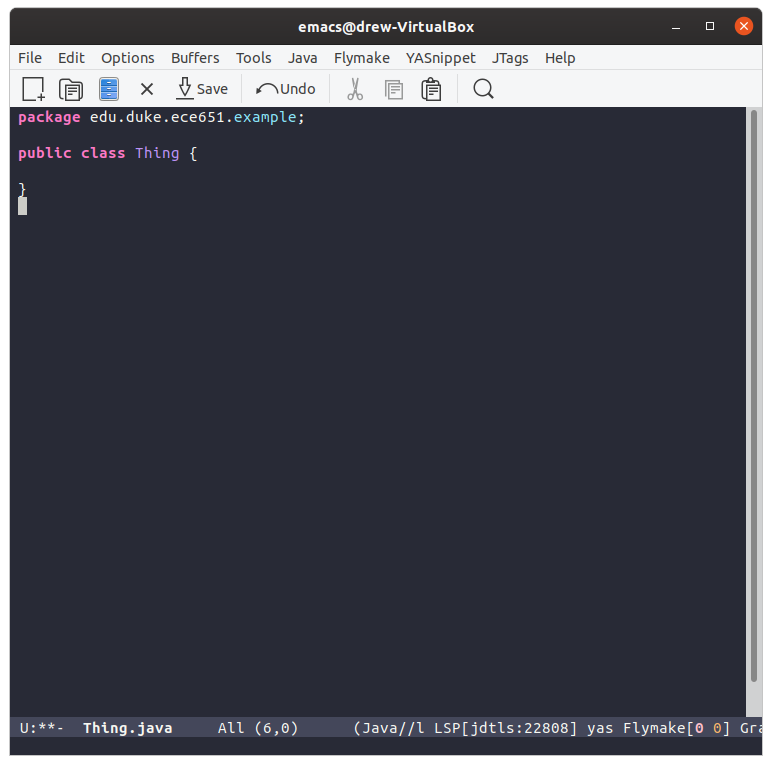
\includegraphics[width=5.5in]{emacs-skel.png}
\end{center}

Note that this has declared the package, and the class, but nothing else.
Lets write some code in it.  First, let us declare a field called \verb+x+:
\begin{verbatim}
  private int x;
\end{verbatim}
And a constructor:
\begin{verbatim}
  public Thing(int x) {
    this.x = x;
  }
\end{verbatim}
And finally a method:
\begin{verbatim}
  public int myFunction(int a, int b) {
    if (a <= 4) {
      return 2 * a + b * x;
    } else {
      return a * x - b;
    }
  }
}
\end{verbatim}

As you type, note that flycheck will complain about anything that is illegal.
When you finish this, we of course need some test cases!

In Java, our testing is structured slightly differently than in C.
For each class X, in the ``main'' source, we are going to write a
testing class XTest in the ``testing'' source.  In this case, our main
class is Test, so we are going to make ThingTest.  We could use C-c
C-f to open the ThingTest file (editing the path to be in the test
part of our source tree), but we have a special key combination to
switch between Java code and its matching test code. Press ``C-x t''
(control x, then t without control).

You should now be looking at ThingTest.java.  Unlike before, this file
is not empty.  The ``C-x t'' command realizes when you are making a new
testing file, and fills it in with an appropriate skeleton.  Note
that this skeleton looks a little bit different. You should see:

\begin{verbatim}
package edu.duke.ece651.example;

import static org.junit.jupiter.api.Assertions.*;

import org.junit.jupiter.api.Test;

public class ThingTest {
  @Test 
  public void test_() {
  }
}
\end{verbatim}


Note that this time, Emacs imported some java packages (that you will
almost certainly need), and created one method with the \verb+@Test+
annotation. When you are using JUnit, you need each of your test
methods annotated with \verb+@Test+.   The method name is not yet completed,
and the point is waiting at the end of the name so you can finish it.
Let's call this method \verb+test_myFunction+.  We'll make this
test case create a \verb+Thing+ object, call \verb+myFunction+ on it,
and check if the result is right.  We use \verb+assertEquals+ to
check that the result is a particular value.  Let us
write the following:

\begin{verbatim}
  @Test
  public void test_myFunction() {
    Thing x = new Thing(3);
    assertEquals(8, x.myFunction(1,2));
  }
\end{verbatim}

Great, we have one test case, so everything is good, right?  Of course not.
First we need to run it, and we probably need some more cases... Hit
``C-c C-t''.   You will get a compilation window while gradle compiles your
code.  When it finishes, you will be presented with a code coverage
report, and see that the lines in your code have been colored
according to if they were covered by your test cases.
When I finish, I see\footnote{Note, after writing this, I configured
  dcoverage to strip off the .java, and also the leading edu.duke.ece651.,
so you won't see those parts of the name.}:
\begin{center}
  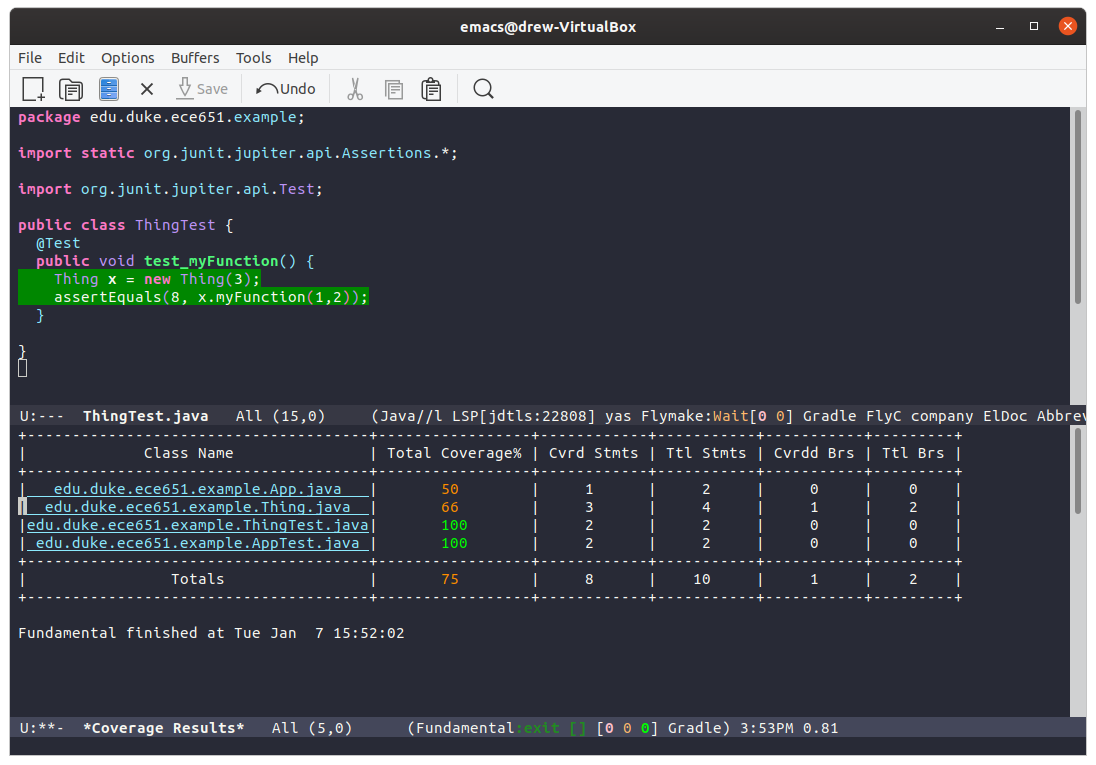
\includegraphics[width=5.5in]{emacs-test-cov1.png}
\end{center}

Note that this report includes the ``App'' and ``AppTest'' classes
that gradle generated (which we haven't done anything with). The
green highlights in the code mean those lines were executed.
Of course, seeing that the test code was executed doesn't help that
much.  We'd like to know about the main code.  In the coverage report,
each of the class names is a clickable link to that particular java
source file.  Put the point on \verb+Thing.java+ and hit enter
\footnote{In theory, a mouse click should work too.  This isn't
  working for me as I write this walk-through.  I will try to fix
this soon, especially if people feel it is important.}.  Of course, you can
still change buffers normally with ``C-x b'' or toggle between main and test
code with ``C-x t''.

Now, you should see something like this:

\begin{center}
  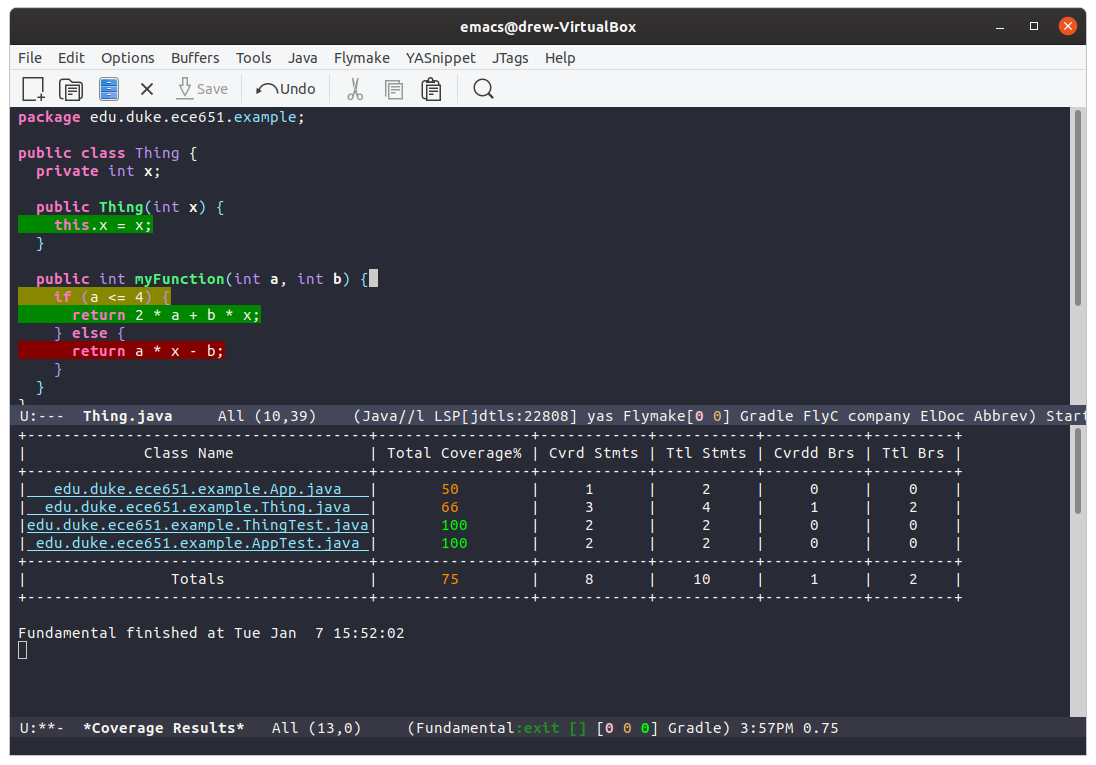
\includegraphics[width=5.5in]{emacs-test-cov2.png}
\end{center}

Note that the various lines of code are colored in three different colors:
\begin{description}
\item[Green] The line of code was covered. For a branch this means you
  covered both directions.  For a non-branch, this means you executed
  that line.
\item[Yellow] This line of code was a partially covered branch.  This
  means that you went one direction of the branch, but not the other.
\item[Red] This line of code was not covered at all.
\end{description}


 If we look at our coverage results for Thing.java, we will see that
 we did not cover the case where \verb+a>4+, so let us write a test
 case where \verb+a+ is 5.

 We'll go back to ThingTest.java (C-x t) and add this to our method:

\begin{verbatim}
    assertEquals(42, x.myFunction(5,6)); 
\end{verbatim}

When you are editing code, you may find having the test coverage
colors displayed annoying.  You can remove them with ``C-c -'' (that is
control c control minus---think of minus for removing things).

Now hit ``C-c C-t'' again to build and run your test cases (if you didn't already save, you will get prompted to).

This time, we get a failed test case:
\begin{verbatim}
example.ThingTest > test_myFunction() FAILED 
  org.opentest4j.AssertionFailedError: expected: <42> but was: <9>
   expected:<40> but was:<39> at org.junit.jupiter.api.AssertionUtils.fail(AssertionUtils.java:55) 
   ...   
   at edu.duke.ece651.example.ThingTest.test_myFunction(ThingTest.java:12)
\end{verbatim}

Note that in reading each test failure, we are most interested in the
first two lines, and the last line.  The first line tells us the class
(\verb+ThingTest+) and method (\verb+test_myFunction+) that failed.  The
next line tells us what in particular failed---usually this is an
AssertionError, which tells us the expected value (42) and the actual
value (9).  The remaining lines are the call stack to get there, with
the deepest calls at the top, and the outermost calls at the bottom.
The last line of this call stack shows us that we called on
ThingTest.java line 12.  That line called assertEquals, which is in
JUnit, and the remaining lines are all inside JUnit.

In this case, our code is completely contrived (just a small made up
example for you to work with your development environment), so what
we do to ``fix'' this doesn't really matter.  However, this
is a great chance to talk about using the debugger.


\subsection{Debugging}
Debugging in Emacs for Java is going to be based primarily around
failed test cases.  That is, we will run a particular test method
(with \verb+@Test+ on it) as the starting point for where execution
of our code in the debugger.

Unfortunately, clover's instrumentation (what it adds to the classes
to figure out our coverage) does not play nicely with the debugger.
Hit ``C-c x'' (not ``C-c C-x'', just ``C-c x'') for ``gradle clean and
compile''.  This will  remove the already built classes, and recompile.

Now we are ready to debug.

To get started, put your point on the line that says
\begin{verbatim}
    assertEquals(42, x.myFunction(5,6)); 
\end{verbatim}

And hit ``C-c C-d''. This command is basically ``start the debugger
for the current test method, and set a breakpoint on the current
line.''  Emacs\footnote{One time I had a problem where it told me it
had no handler for resolving the classpath. Restarting Emacs fixed
this.} will take few seconds while it starts up the debugger (you may
see a window or two flash up and vanish---this is no big deal).  When
everything is ready, you should see:


\begin{center}
  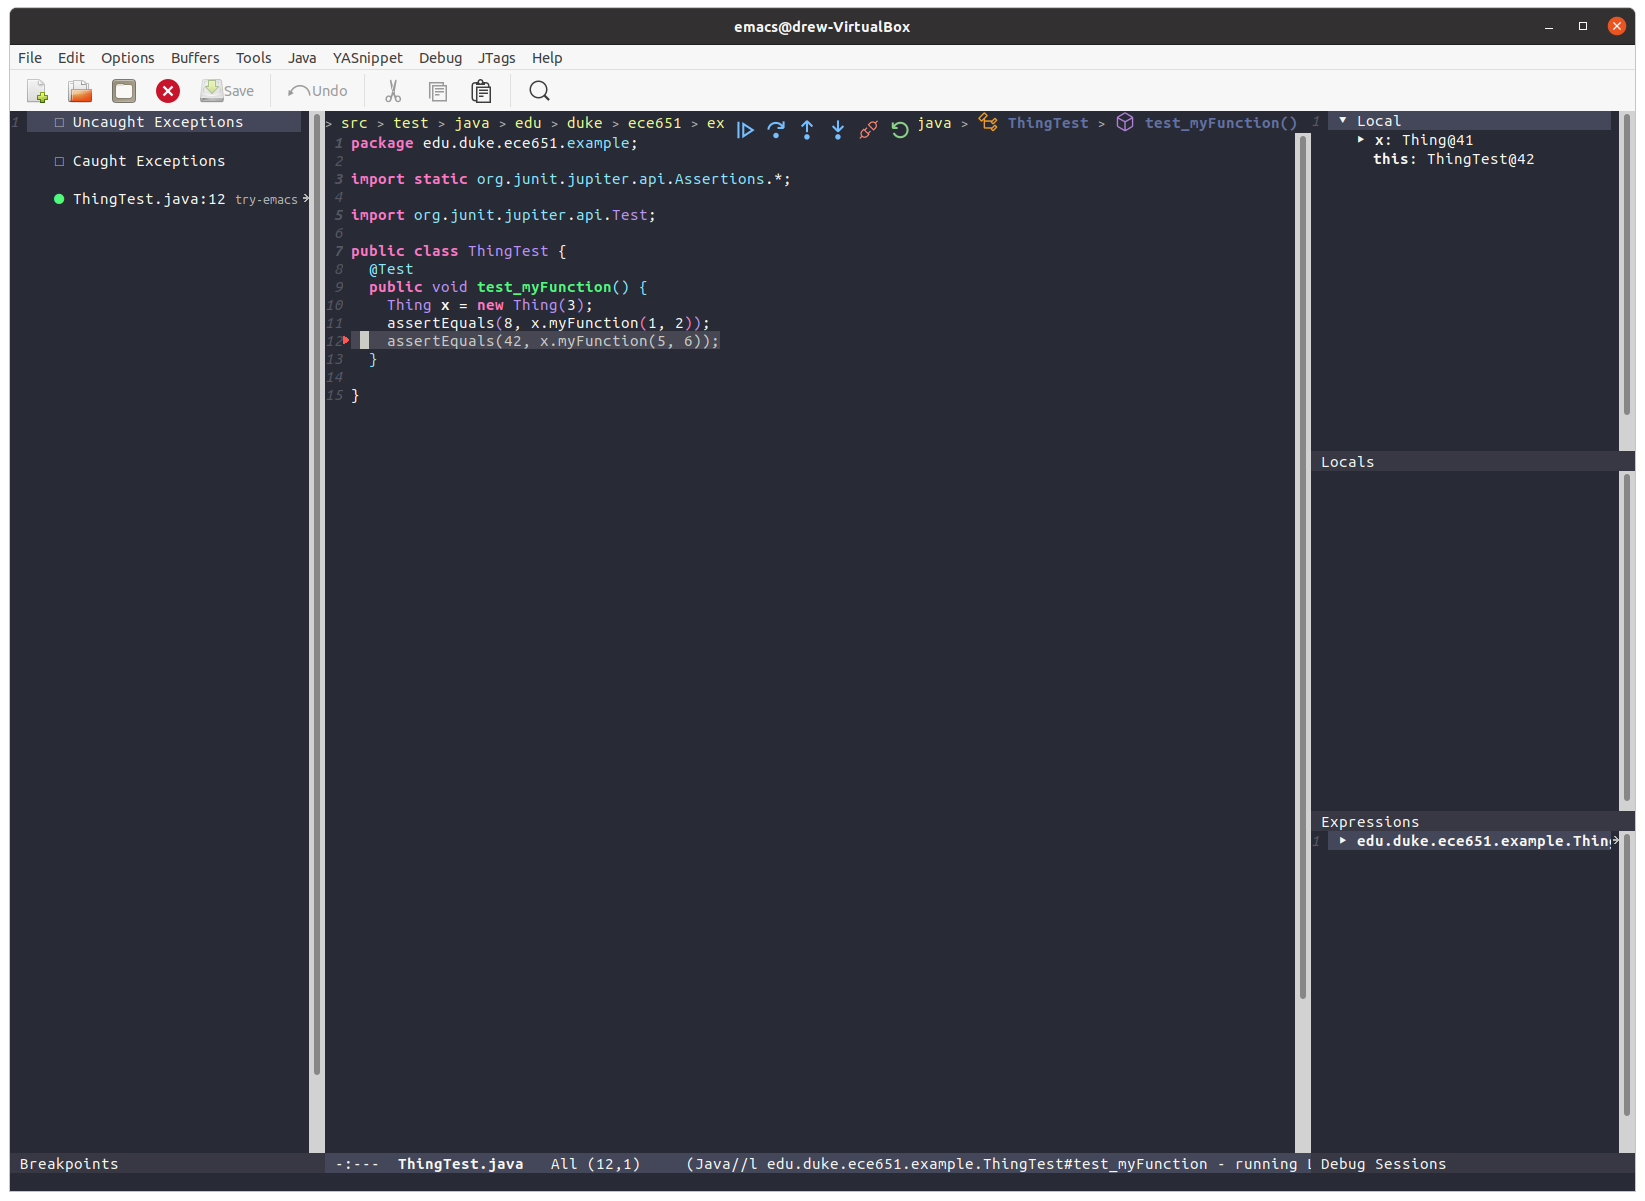
\includegraphics[width=5.5in]{emacs-debug1.png}
\end{center}

The middle part shows your code, with execution stopped at the breakpopint on the assertEquals (set
by hitting C-c C-d).  The left shows some things related to exceptions (which we won't go into here).
On the right, you should have Local variables at the top, and a few other things below it.

If you are running in a graphical emacs, there will be a small row of
buttons at the top to continue execution, step over the current
statement, go up a frame, step into the current call, disconnect the
debugger, or restart\footnote{If you use this, it will display an
extra window with the debugger process.  You can hide that with C-x
0.}.  You should also have a hydra visible at the bottom of the
window.   A hydra is basically a different remapping of keys.  While the
hydra is open, the keys that it lists will behave differently.  You can use
C-c C-h to toggle whether the hydra is active.  

You should be in the main code window (if not, go back into it).  Either hit
the ``down arrow pointing at a dot'' button if you prefer the graphical buttons, or
if you are using the hydra, hit 'i' (for step in).

This should step inside the call to myFunction. Emacs will change to
displaying Thing.java, and the execution will be in the start of
myFunction.  Note that the local variables on the right also changed.
Of course, now \verb+this+ is our Thing object, which has \verb+x=3+.
You can see that if you expand \verb+this=+ on the right.

Now, let us go to the next line.  If you are using the hydra, hit \verb+n+. If
you are using the buttons at the top, hit the one that looks like an arrow
arcing over a dot. Now we are on the line of code that computes
the return value.  In gdb, you would use ``print'' (or ``p'') to see
the value a variety of things.  Here, you are going to use one of the
``e'' commands on the right of the hydra (there is no equivalent to this
in the buttons---the hydra provides many more options).

You can use ``er'' (Eval region) to evaluate an expression in a region
you have selected.  Set the mark 
at the start of the expression, then move the point to the end.  Now hit ``er'' (with the hydra
active).  If you do this on the expression \verb+a*x-b+ in this code,
you will see $=> 9$ showing you that this expression
evaluates to 9 (right next to it).  You can see this behavior here:

\begin{center}
  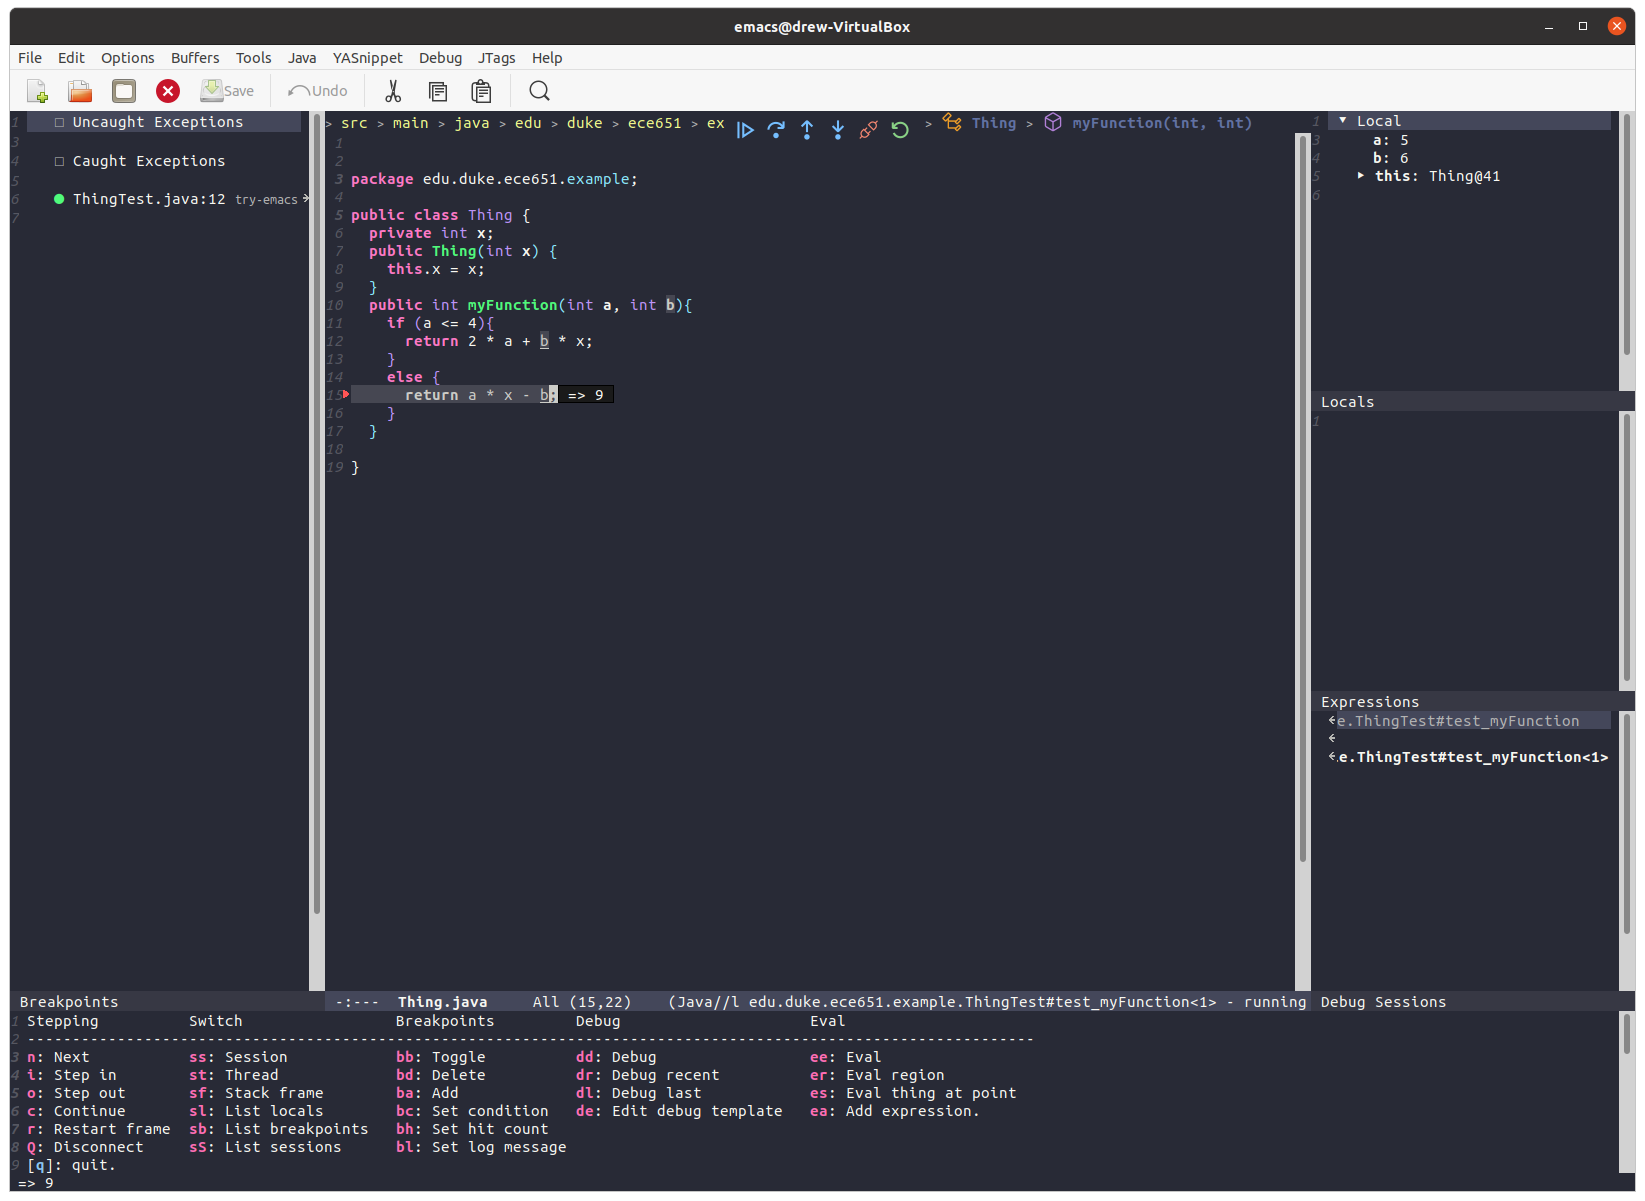
\includegraphics[width=5.5in]{emacs-debug-er.png}
\end{center}

Many of the other commands are familiar, even if by a slightly
different name.  The ``o'' command (step out) is ``finish'' (run until
the current function returns).  There are a variety of breakpoint
commands in the ``Breakpoints'' column.
When you are done debugging hit ``Q''.

One thing about the ``hydra'' is that it is great when you want those
keys to control the debugger, but terrible if you want to do anything
else (like change buffers, edit code, etc), as the hydra intercepts
those key strokes.  You can pause/resume the hydra with C-c C-h (the h
is for hydra). Note that you will be reminded of this as the debugging
starts. So pause the hydra whenever you want to do anything else.
You can also hide the hydra with ``q''.  If you want to quit the debugger,
use 'Q' in the hydra, or the ``disconnect'' button at the top (it looks like
an orange plug being pulled out).

Let us wrap this ``Debugging'' up by ``fixing'' our contrived code
by adding ``+33'' to the end of that line:
\begin{verbatim}
  return a * x + b + 33;
\end{verbatim}

Now press ``C-c C-t'' again to see test coverage.   At this point, we should
have 100\% coverage on Thing.java, and all the lines turned green--yay!


\subsection{Having Emacs Do The Boring Stuff}
So far, you have not needed to import any other packages (other than
a few that were automatically setup for JUnit).  However, as
you develop with Java, you are going to find that you generally import
many many packages.  Let us write some code that needs to have
an import from java.util.  Go into Thing.java, and add another method:

\begin{verbatim}
 public int computeStuff(ArrayList<Integer> a, 
                         ArrayList<Integer> b) {
}
\end{verbatim}

As you type this, you will notice that flycheck puts a red underline
under ArrayList\footnote{ArrayList is like std::vector from C++. Java
  also has Vector.  The difference is that Vector locks a mutex for
  each method.  Unless you need the mutex, use ArrayList.}, and a red
\verb+>> + on the left of the buffer to show you the problems. If you
rest the point on the word ArrayList, you will get the message from
flycheck that ``ArrayList cannot be resolved to a type''.

You can have Emacs import the packages that you
need by hitting C-c TAB. You will see that your code got modified
to have  
\begin{verbatim}
import java.util.ArrayList;
\end{verbatim}
at the top. That is great, but flycheck is still unhappy with our method.
If you rest the point on any of the underlined code, you will see that
it is because we need to return an int, and we don't return anything yet.

While we are at it, let us take a moment to have Emacs open up the
Javadoc (documentation) for ArrayList. Put the point on the word
ArrayList, and press ``C-c C-j''.  You will get prompted for the
class name you want to lookup, with java.util.ArrayList at the first
and in bold. Hit enter, and your default browser (likely Firefox) will
load the page with the documentation for ArrayList. Note this might
take a second as Firefox loads.  After finding the methods
that we need from this documentation, we write:

\begin{verbatim}
  public int computeStuff(ArrayList<Integer> a, 
                          ArrayList<Integer> b) {
    int temp = 0;
    for (int i = 0; i < Math.min(a.size(),b.size()); i++) {
      temp += a.get(i) * b.get(i);
    }
    return myFunction(a.get(0), b.get(0)) * temp;
  }
\end{verbatim}


Before we move on, we think ``hey, maybe we should pull that first bit
of code out into its own method, since it computes a dot product.. we
might want to do that again''.  Fortunately, Emacs can do this for you.
Select that region of code:

\begin{center}
  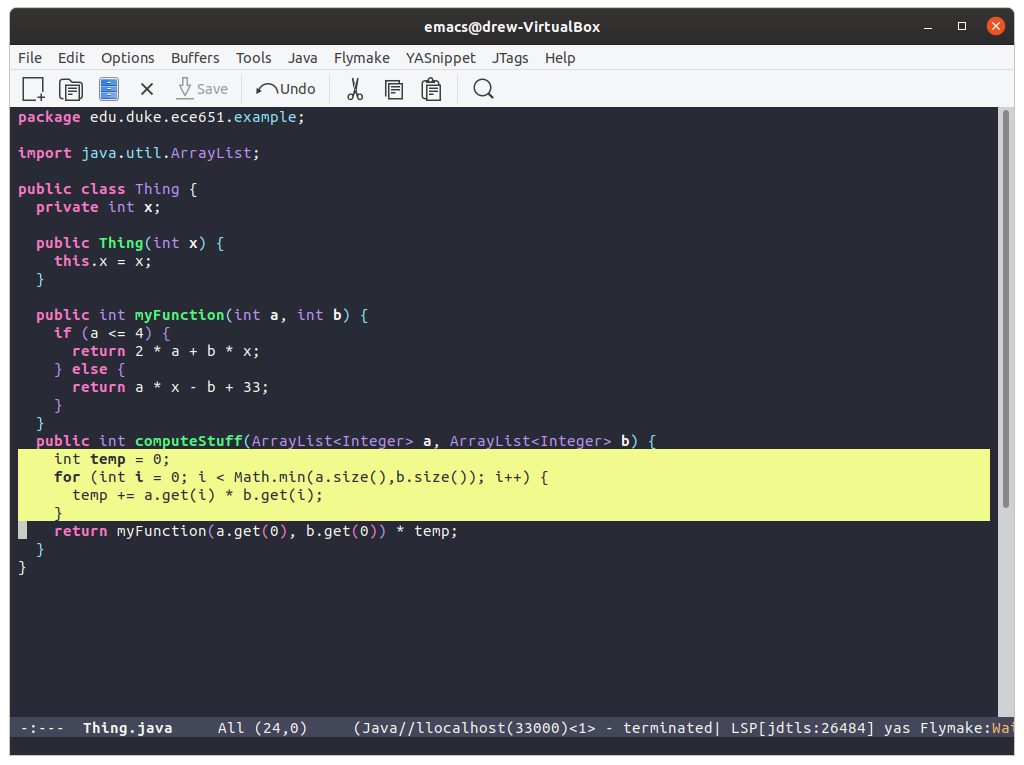
\includegraphics[width=5.5in]{emacs-em-pre.png}
\end{center}

Now hit ``C-c C-e'' (the e is for extract method).  Emacs will prompt
you for the name of the extracted method (the default is
``extracted''---lets change that to ``dotProduct'', then hit enter).

Now you should have code that looks like this:

\begin{center}
  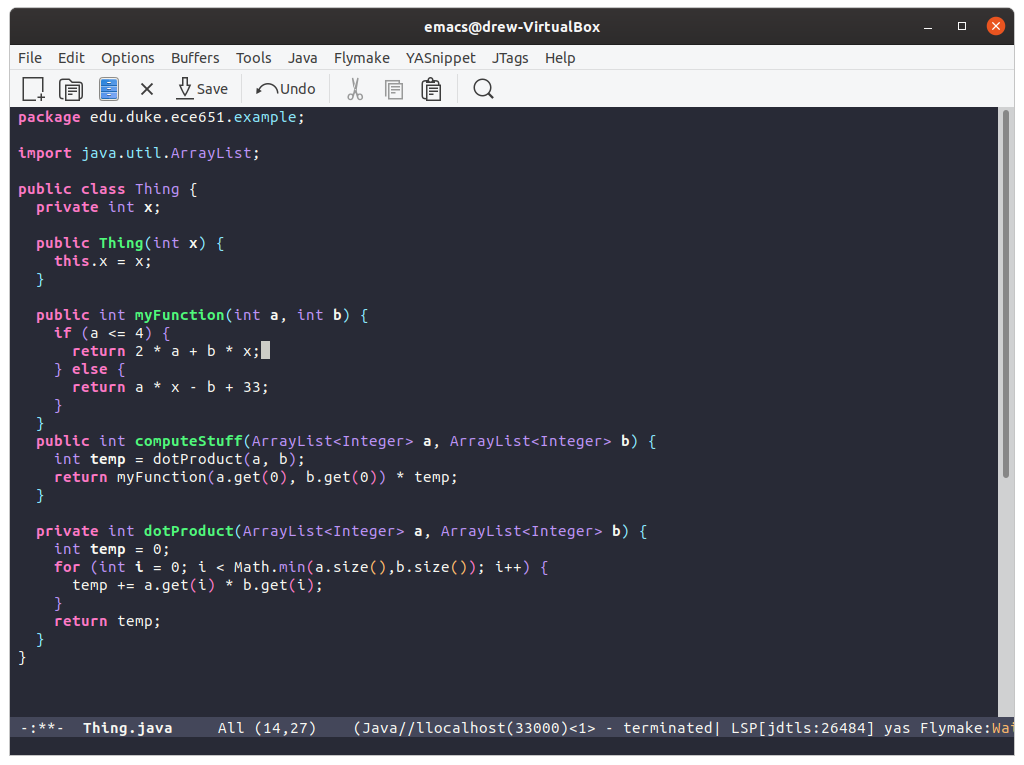
\includegraphics[width=5.5in]{emacs-em-post.png}
\end{center}

Note that if your code has syntax errors, extract method will not work.
The error message you get will be a little misleading, as it says that the
operation is unsupported.

Before we proceed, our code needs to be tidied up. Hit C-c C-f to autoformat
the code.

At this point, you can write a test case of your own for this method!
Go back to the ThingTest.java class (C-x t), and add a new method. Write
one or more test cases in this method.  Note that you will need to use
\verb+new+ to make ArrayLists.  You might want to look in the Javadocs
to find how to add items to the ArrayList. When you are done, run
your test cases and look at your coverage.

Next, let us see how to auto-generate method stubs for
methods that are required by an interface or abstract parent class.
Let us start by making an IntRangeEnumeration class.  Create
IntRangeEnumeration.java in the \textbf{main} source directory (inside
the example package).  The easiest way to make sure you create this in the
right place is to go back to Thing.java (which is in the directory you want)
and C-x C-f from there. Remember that you can create the skeleton
of this class with ``C-c C-s''.  
Now add \verb+implements Enumeration<Integer>+ after the class name.
Once you do that, you should have this:

\begin{verbatim}
pubic class IntRangeEnumeration implements Enumeration<Integer> {

}
\end{verbatim}

notice that Enumeration is underlined in red.  We need to import something,
so we hit C-c TAB.

After that import is added, you will see that IntRangeEnumeration is
underlined. The error now is that our class has to implement the
methods that the interface requires (``implement the inherited
abstract method XXX'').  With the point anywhere on the method
declaration line, hit ``C-c C-a'' (the a is for ``add'') to add stubs
for the unimplemented methods. Now you should see:

\begin{center}
  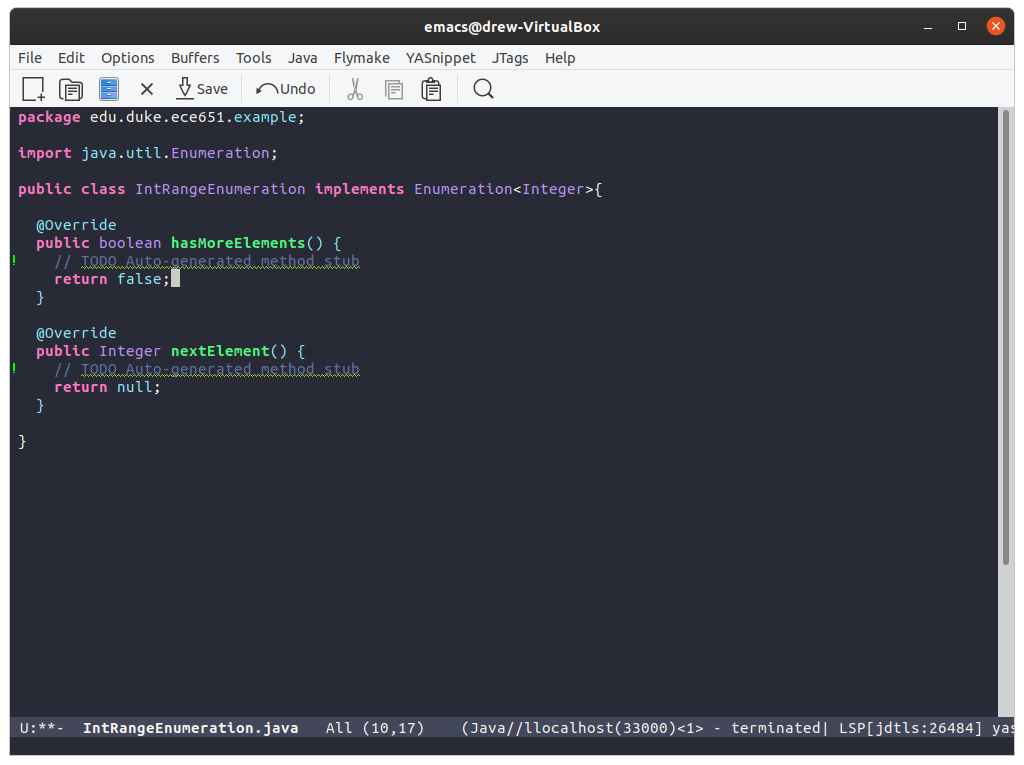
\includegraphics[width=5.5in]{emacs-add-method.png}
\end{center}
Note that there are green exclaimation marks on the lines with TODO comments.
These are there to make it easier to find things marked with TODO.
Also note that these methods have the \verb+@Override+ annotation.

What do these methods need to do?  Our idea for this class is that it
should enumerate integers in a range.  To see how that works with the
methods required by the Enumeration interface, remember we can put the
point on Enumeration and hit ``C-c C-j'' to read its Javadoc.

Accordingly, we might write:

\begin{verbatim}
public class IntRangeEnumeration implements Enumeration<Integer>{
  private int current;
  private int max;
  public IntRangeEnumeration(int low, int high) {
    this.current = low;
    this.max = high;
  }
  @Override
  public boolean hasMoreElements() {
    return current < max;
  }

  @Override
  public Integer nextElement() {
    if (current >= max) {
      throw new NoSuchElementException("No more elements in range");
    }
    int temp = current;
    current++;
    return temp;
  }

}
\end{verbatim}

We again see that NoSuchElementException needs an import, so we
hit C-c TAB to have Emacs automatically import it.

Of course, now you should create a test class (remember that C-x t will
make the right file, and create the skeleton for a JUnit test for you),
write some test cases, and run them.  Are you happy with this code?

You can also have Emacs generate one particular method override from a
parent class (``C-c C-o'' the o is for override--you will be prompted
to select which method to override) and getters/setters for a class
(``M-g g'', that is ESC g g---the g g is for ``generate getters'').
However, use the last with care.  If you find yourself often making
classes that expose many of their fields through getters/setters, you
are probably doing something wrong in terms of design.
If you use the generate getters/setters and have multiple fields
that do not yet have getters and setters, you will get prompted for which
one(s) you want.  If you just want one, cursor down to the desired one and
hit enter.  If you want to select a few, go to the ones you want, and hit
C-space on their lines.  If you want all visible candidates, hit M-a to
select all (you could select all then deselect a few). One you have the right
selections, hit enter.  If you have many selections to choose from, you can start
typing the name of the field you want to narrow down what is shown.



\subsection{Peeking}
If you want to find the place(s) that something is defined or used
(referenced), then you can ``peek'' at them with ``C-c d'' (for
definitions) and ``C-c u'' (for uses).  Note that both
of these don't have control on the second character.
Peeking at them means that emacs
will put up a couple smaller windows. The right one will
show you the files and the places in them that the definitions/uses are
found (expand/collapse the files with enter).  The left will show you
the code around that definition/use.

%% For example, if I put the point on myFunction (in \emph{e.g.}, ThingTest),
%% and hit ``C-c u'', then I will peek for all uses of myFunction, like this:
%% \begin{center}
%%   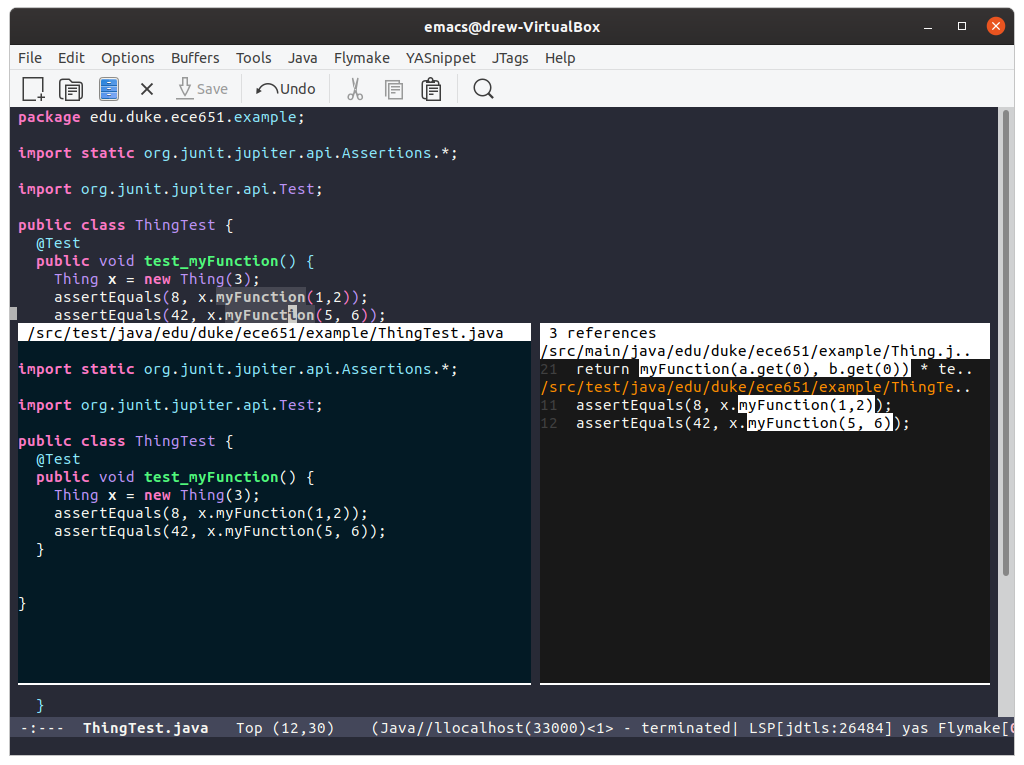
\includegraphics[width=5.5in]{emacs-peek.png}
%% \end{center}

%% The bottom part of Emacs is showing the ``peek'' view\footnote{Moving
%%   the mouse seems to close the peek view.  This is surprising to me,
%%   but only came up in writing this walk-through, since I primarily use
%%   the keyboard.  I'm looking for a workaround.  In the meantime, use
%%   the keys to navigate the peek.}.  On the right is a list of the
%% places that myFunction is used.  The orange lines are the filenames,
%% and the white lines under them are the particular lines of code.  Each
%% of the file names can be expanded/contracted by putting the point on
%% it and hitting enter.  As you move the point onto the various uses
%% ,the display on the left will change to show you that particular use
%% in the code.

If you hit enter on a particular use, you will stop peeking and
switch your main code to view that use.  If you want to stop peeking
and stay where you are, just hit C-g (which you should remember
from 551 cancels most things in Emacs).

\section{Upping your Emacs/Git Game}
At this point, you have the basics of your Java development setup.
You should be able to work on your assignments in this class in Emacs
and have all the basic features you need (if you want more, install
the appropriate packages!).  However, you may wish to have better
git/Emacs integration.  In this section, we will give you a quick
introduction to \verb+magit+, a powerful package that integrates git
with Emacs.  Later in the semester (when you start working in teams),
we will come back and show you how to use \verb+forge+ (which works
with magit) to integrate with GitLab's issue tracking/code review/pull
request features.  If you don't want to use git inside of emacs, you
can continue to use it on the command line, and can do all of the
issue tracking/code review/merge request activities from the GitLab
website.

Before you start, we recommend that you do the following command:
\begin{verbatim}
git config --global status.showUntrackedFiles all
\end{verbatim}


To start, hit ``C-c g'' which opens the magit status buffer.  This
buffer is where you will work from for most git things you need to do.
This buffer will have various section for ``Untracked files'',
``Unstaged changes'', ``Staged changes'', etc.  If you have
been following along, you have many untracked files inside of
the ``try-emacs'' directory.   Magit will show that directory
as something expandable/collapsable.  If it is collapsed,
move the point onto it and hit TAB. You should add things like
build.gradle, and the src directroy (adding src will add all files
inside it), but not things like ``build'' which were generated by gradle.

To add a file (or directory), move the point
onto the line for that file in Unstaged changes list.   Now hit ``s'' to stage
You will see that it got moved to ``Staged changes''.   Note that
this action was basically like doing ``git add'' on that file.
If you want to unstage this change, you can move the point onto the
line for that file in the Staged Changes section and hit ``u''.

Let us suppose that you want to check exactly what you changed before
you commit this change.  Move the point onto the line for the file and
hit TAB.  In magit, TAB is expand/collapse.  For a file with changes,
expanding it shows the differences---things that were removed are in
red with a - at the front, and things that were added are in green
with a + at the front.  You can collapse the changes back with TAB
again.  You can also use TAB to expand/collapse other things, like
each of the sections (if you put the point on the section name).
In our current situation, this is not super useful, as the changes
are all ``created the entire file''---but as you develop larger
pieces of software over the semester, this will be a great feature.

Now let us commit our changes.  Hit ``c'' in the magit status buffer.
It will pop up a window at the bottom with various options and types
of commits you can make.  We want to make just a plain ordinary
commit, so hit ``c'' again.  You will now end up with the differences
showing on the left, and the commit message on the right.  Go ahead
and write a commit message\footnote{I know many of you wrote really
  bad commit messages in 551.  Now is the time to get in the habit of
  writing good ones, since you are about to work in teams...}(such as
``Wrote test cases for the Thing class: reached 100\% coverage'').
Unlike 551 where you would save and quit, when you are done, hit C-c
C-c.  This will finish the commit message and have magit make the
commit.

Now, we'd like to push (assuming you forked the repo, instead of just
cloning it).  To push, hit ``P'' (case matters) and you will see a
window at the bottom for various push options.  We want to just push
to origin (where we cloned from), so hit ``u''.  You will then see
\begin{verbatim}
Running git push -v origin master:refs/heads/master
\end{verbatim}
and if there are no problems, after a little while, it will switch to
\begin{verbatim}
Git finished
\end{verbatim}

Of course, the other major operation you will want to do at this point
is \verb+git pull+.  To do that, hit ``F'' and you will get the window
for git pull.  Hit ``u'' to pull from origin, and you will see similar
messages as with pushing.

For quick reference on magit commands, please see:
\url{https://magit.vc/manual/magit-refcard.pdf}

\section{New Feature Quick Reference}
\label{Sec:QuickRef}

\textbf{Generating Things}
\begin{verbatim}
C-c C-s Create class skeleton
C-c TAB Add missing imports
C-c C-a Add unimplemented methods
C-c C-o Add override
M-g g Add getters/setters
\end{verbatim}
\noindent\textbf{Changing Things}
\begin{verbatim}
C-c C-e Extract method (from selected region)
C-c r   Rename symbol at point
C-c C-f Format buffer
\end{verbatim}

\noindent\textbf{Testing + Debugging}
\begin{verbatim}
C-x t   Switch between main and test code
C-c C-t Run tests and show coverage
C-c -   Remove coverage colors
C-c C-d Debug current test method with breakpoint at point
C-c C-h Pause/resume debugger hydra
\end{verbatim}

\noindent\textbf{Gradle Build}
\begin{verbatim}
C-c C-v Gradle build
C-c x   Gradle clean + build
C-c C-r Gradle build + run
\end{verbatim}

\noindent\textbf{Finding Things}
\begin{verbatim}
C-c C-j Javadoc lookup
C-c u   Peek at uses
C-c d   Peek at definitions
C-c i   Goto implementation (of method at point)
C-c t   Goto type definition (of type name/var name at point)
        (for variables: goes to definition of its static type)
\end{verbatim}
\noindent\textbf{Git}
\begin{verbatim}
C-c g   Magit status buffer
\end{verbatim}
\newpage
\section{Customizing Emacs}
We've tried to set you up with a good base setup, however,
you  may want to customize a lot of things. Feel free!  If you
have particularly nice customizations, or packages you really like,
post them on Piazza.  If something is very popular, we will consider
including it in future setups.

\subsection{Themes}
If you do not like the Dracula theme that we picked, there
are many other themes to choose from.  You can start by looking
at \url{https://emacsthemes.com/popular/index.html}.
If you find a theme that you like, go into Emacs and hit
\begin{verbatim}
M-x list-packages
\end{verbatim}

Give the package list a moment to load, then his C-s to incrementally
search, and start typing the name of the theme.  When you find it, click
it and click ``install''.  Then edit your \verb+~/.emacs+ file,
and find
\begin{verbatim}
(load-theme 'dracula)
\end{verbatim}
at the end.  Change that to the name of the theme you installed.  Your
changes should take effect when you start Emacs.

\subsection{Customization variables}
If you hit \verb+M-x customize+ you will get the Emacs customization
interface.  Many packages provide a wide array of customizable settings.
For example, if you change your theme and find that the code coverage
coloration does not work well with your theme's colors, you might
want to change the code coverage colors.  The code coverage is provided
by the dcoverage package, so type do \verb+M-x customize+ then
type ``dcoverage'' into the search box.  The first option will be
``dcoverage covered statement color'', which is the color for statements
that got covered.  If you expand this, you will see that it has the
color (written as a hex value) and a ``Choose'' button.  If you press
the Choose button, you can select from about 500 pre-defined colors.
You can, of course, also write in an RGB value in hex if you prefer.


\subsection{Key bindings}
We tried to set up a variety of useful key bindings.  However, if you
have other features you use often, or if these clash with key bindings you
setup in 551 that you want to keep using, you can change them.
Some key bindings are provided by packages (e.g., ``C-c C-t'' is
provided by dcoverage) and may be customizable through \verb+M-x customize+.
Others we setup in the Java mode hooks, so just edit your \verb+.emacs+ file
and look for the \verb+local-set-key+ commands in the Java mode hook.

\subsection{Dcoverage}
If you have feature requests for dcoverage, post them on Piazza.  If they
seem good, I'll implement them as time permits.

\end{document}
